\begin{figure}
    \centering
    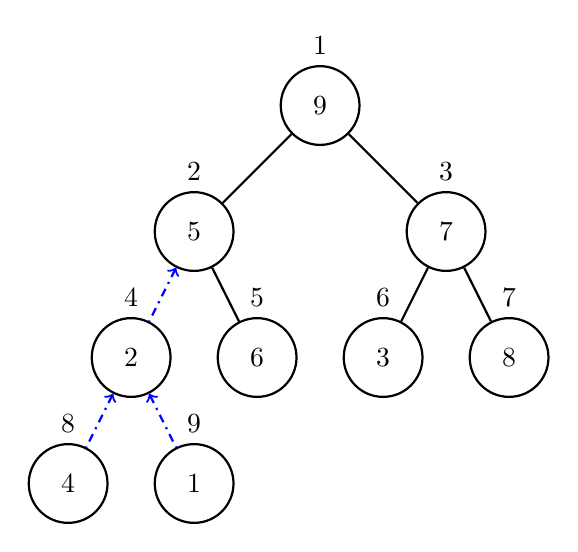
\begin{tikzpicture}[thick, scale=0.8]
        \node[label={1},circle,draw,minimum size=1cm]
            (1) at (0,0) {$9$};
        \node[label={2},circle,draw,minimum size=1cm]
            (2) at (-2,-2) {$5$};
        \node[label={3},circle,draw,minimum size=1cm]
            (3) at (2,-2) {$7$};
        \node[label={4},circle,draw,minimum size=1cm]
            (4) at (-3,-4) {$2$};
        \node[label={5},circle,draw,minimum size=1cm]
            (5) at (-1,-4) {$6$};
        \node[label={6},circle,draw,minimum size=1cm]
            (6) at (1,-4) {$3$};
        \node[label={7},circle,draw,minimum size=1cm]
            (7) at (3,-4) {$8$};
        \node[label={8},circle,draw,minimum size=1cm]
            (8) at (-4,-6) {$4$};
        \node[label={9},circle,draw,minimum size=1cm]
            (9) at (-2,-6) {$1$};

        \tikzstyle{cert}=[<-, dashdotted, blue, thick]
        \draw[thick] (1) -- (2);
        \draw[thick] (1) -- (3);
        \draw[cert] (2) -- (4);
        \draw[thick] (2) -- (5);
        \draw[thick] (3) -- (6);
        \draw[thick] (3) -- (7);
        \draw[cert] (4) -- (8);
        \draw[cert] (4) -- (9);
    \end{tikzpicture}
    \caption[Certificados após \textsc{change}]{Após a mudança de
    velocidade do elemento 2, que se encontra em \heap[$4$],
    \cert[$4$], \cert[$8$] e \cert[$9$] foram atualizados.}
    \label{fig:predeventheap}
\end{figure}